%   Filename    : chapter_4.tex 
\chapter{Research Methodology}
This chapter lists and discusses the specific steps and activities that will be performed  to accomplish the project. 
The discussion covers the activities from pre-proposal to Final SP Writing.

\section{Research Activities}
This project aimed to create an automated attendance system with the help of RFID together with facial recognition technology. This attendance system will replace and reduce the usage of manual attendance such as the written and oral and enhance its lacking optimized features such as security, reliability, authenticity, and integrity using the student’s RFID and facial biometric.

The proposed system is expected to function by tapping the RFID of the students with real time facial capture through face recognition technology. The identity of the students will be verified through the unique serial number of their RFID that will match from the system database while the face recognition will serve as the two-factor authentication. The face recognition is expected to work by capturing the students face then will be matched also through the system database. The attendance will only be valid once both student’s unique serial number in their RFID and their face has been verified.

To make the system functional, several data from the students need to be collected. Those are the student’s name, student number, student’s unique serial number of  their RFID, and their facial biometrics. Those data will be gathered either online or face to face. Students are encouraged to download any of the RFID card readers to know their RFID’s serial number but in case they are incapable of doing that. Face to face to face will be an option where we can provide a physical RFID card reader. The facial recognition data will be gathered through capturing their image or video to be more accurate. 

The hardware components will be using in this system are:
RFID scanner: Which will be used to read the RFID given to the students. This will also be responsible for taking the students unique serial number on their RFID ensuring the integrity of the students.
USB connector: This will be used to connect the RFID scanner to the Laptop or Raspberry Pi. Flex cable: This will be used to connect the Raspberry Pi Vision Camera to Raspberry Pi.
Laptop / Raspberry Pi: This will serve as the main processing unit. The laptop or raspberry pi will be used for running the required algorithm to make the face recognition and read the RFID correctly. Overall, the laptop / raspberry pi will be in charge of handling the data.
Raspberry Pi Vision Camera: In charge of capturing the student’s facial image while scanning the RFID to the RFID scanner. 

\section{RFID and Face Recognition}
 We use the UP RFID for our system. This approach enhances security by combining something you have (the RFID token) with something you are (your face).
 \subsection{RFID as a Token}
 The RFID token (the UP RFID) provides a unique identifier (ID) for the user. The RFID reader scans the token and extracts the unique ID. This ID is used to retrieve the corresponding user profile from a database.
 \subsection{Face Recognition as a Verifier}
  Face recognition ensures that the person presenting the RFID token is the authorized user associated with that token.
 	
\section{Face Recognition}
Face recognition pipeline can be simplified into 2 steps:
\begin{enumerate}
	\item Face Detection: The process of finding the faces in a viewfinder and draw bounding boxes around the detected face. We will use a pretrained YOLOv8n model
	as the base model for face detection.
	
	\item Face verification: This is a downstream task from face detection. We will use the cropped image from as input for the face recognition model to identify the individual. It is based on the same pretrained YOLOv8n model fine tuned for identifying faces. We used the YoloV8n as it is the only supported by YOLO toolkit to be exported to IMX500 chip. Also, 'n' means nano or the smallest model in the YoloV8 family of models as larger models like the YoloV8m are not able to fit to the 8mb memory of IMX500 \cite{sony_imx500}.
\end{enumerate}
\subsection{Face recognition model training} 
Fortunately, Ultralytics(the team behind the YOLO model) provides complete documentation for finetuning a pretrained model using few lines of code. The data.yaml file contains the dataset information such as the directory of the images and their corresponding labels. The model can then be exported to the Sony IMX500 vision sensor for inference\cite{ultralytics_yolo_docs_2024}. 
\begin{figure}[h] % 'h' places the figure approximately here in the text
	\centering
	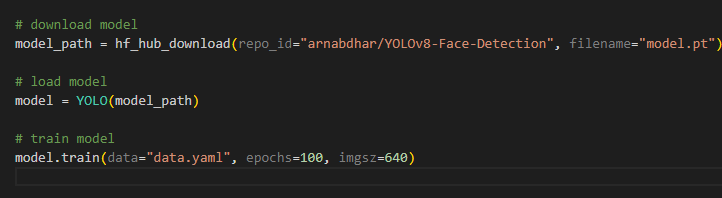
\includegraphics[width=1\textwidth]{figures/chapter3/train.png} % Adjust width as needed
	\caption{Training the model}
	\label{fig:api}
\end{figure} 


\section{Hardware Development Tools}
Our current prototype uses hardware components that are commonly used in the industry to build an integrated system. All of the tools are readily available. These include but are not limited to:

\begin{itemize}
	\item	RFID Scanner - Used as a reader for the RFID. The RFID scanner allows us to have secured and efficient way of identifying the student's unique serial number.

\end{itemize}

\begin{itemize}
	\item	Raspberry Pi AI Camera - The newly released camera module for Raspberry Pi hardware that allows us to capture the student's facial image while scanning the RFID with the use of RFID scanner. It uses an embedded AI accelerator for efficient processing of face data.
	
\end{itemize} 

\begin{itemize}
	\item	Raspberry Pi - Serves as the main processing unit which allows us to integrate the other hardware together with the necessary software.
	
\end{itemize}

\begin{itemize}
	\item	USB Connector -  Serves as connector for the RFID scanner and Raspberry Pi.
	
\end{itemize}

\begin{itemize}
	\item	Flex Cable -  Serves as connector for the Raspberry Pi Vision Camera and Raspberry Pi. 
	
\end{itemize}
	
\section{Software Development Tools}
\label{sec:devtools}
 Our current protoype include these frameworks and tools that are heavily used in the industry for rapid development and deployment of web applications. All of the tools used are open source. These include but are not limited to:
 
\begin{itemize}
	\item	Django - The web framework for perfectionists with deadlines. Django, which serves as the backend server, allows us to interface with the database server to do queries in the Python using Django's Object Relational Mapping tool(ORM). We can easily integrate popular pretrained facial recognition models as they are typically written in Python.
\end{itemize}

\begin{itemize}
	\item	Django Ninja - Creates the REST API on top of our Django backend to allow the frontend to consume the backend content.
\end{itemize}

\begin{itemize}
	\item	NuxtJS - The frontend JavaScript framework used to build our web interface. Includes all the tools for routing, quering, and security. By default, it renders our web interface in Server Side Rendering(SSR) mode. Most of the work happens in the server and no authentication tokens are stored in the client browser. This increases security since authentication tokens are only added in the server side per request.
\end{itemize}
	
